\documentclass[a4paper]{article}

\usepackage[english]{babel}
\usepackage{amsmath}
\usepackage{amssymb}
\usepackage{dsfont}
\usepackage{tikz}
\usepackage{framed} 
\usetikzlibrary{arrows,automata}
\title{Calculus and Probability Theory\\ Assignment 5}
\author{Christoph Schmidl\\
s4226887\\
Data Science\\
c.schmidl@student.ru.nl\\}
\date{\today}


\begin{document}
\maketitle





\textbf{After completing these exercises successfully you should be confident with the following topics:}

\begin{itemize}
	\item familiar with definite and indefinite integrals
	\item able to apply the most important integration methods, more specifically, substitution and integration by parts
	\item confident about switching between different representations of a function
	\item able to compute area of a finite or infinite region
	\item able to apply the formula for the arc length of a function over a finite interval
\end{itemize}
\vspace{1em}

\begin{enumerate}


%%%%%%%%%%%% Task 1 %%%%%%%%%%%%
\item (\textbf{20 points}) Compute the following indefinite integrals. You can use \textit{substitution} or \textit{integration by parts}. In each problem \textit{verify} your result, and don't forget about the constant term. You may need some of the following, well-known trigonometric identities:

\begin{align}
	\sin(2x) = 2\sin(x)\cos(x), \quad \cos(2x) = \cos^2(x) - \sin^2(x), \quad \sin^2(x) + \cos^2(x) = 1\notag
\end{align}

Also, it is highly recommended to consult with the lecture slides and solve the problems there before you start with these ones.

\begin{enumerate}
	%%%%%%%% Task 1.a %%%%%%%%
	\item $\int \sin(x) \cos(x) \; dx$\\
	\textbf{Solution:}\\

Applying substitution seems to be the best approach here. Note: everytime a factor in the integrand is a derivative of the other factor in the integrand, it is a good idea to use substitution instead of integration by parts.

Substitution

\begin{align*}
	\int_a^b f(u(x)) \cdot u'(x) dx = \int_{u(a)}^{u(b)} f(u) du
\end{align*}


Let $u = \sin(x)$. Then $du = \cos(x)dx$. So, $dx = \frac{du}{\cos(x)}$

\begin{align}
	\int \sin(x) \cos(x) \; dx &= \int u \cos(x) \frac{du}{\cos(x)}\notag\\
	&= \int u \; du\notag\\
	&= \frac{1}{2}u^2\notag\\
	&= \frac{1}{2} \sin^2(x) + C\notag
\end{align}	

	
	
	%%%%%%%% Task 1.b %%%%%%%%
	\item $\int \ln(ax) \; dx$ where $a > 0$\\
	\textbf{Solution:}\\
	
Integration by parts

\begin{align*}
	\int_a^b u(x) \cdot v'(x)dx = \left[ u(x) \cdot v(x) \right] - \int_a^b u'(x) \cdot v(x)dx
\end{align*}

	
\begin{align*}
	\int \ln(ax) \; dx &= \int ln(ax) \cdot 1 \; dx
\end{align*}

Let $v' = 1$ and $u = ln(ax) \rightarrow v = x$ and

\begin{align*}
	u' = (ln(ax))' = \frac{1}{ax} \cdot a = \frac{1}{x}
\end{align*}

\begin{align*}
	\int ln(ax) \cdot 1 \; dx &= \left[ ln(ax) \cdot x\right] - \int \frac{1}{x} \cdot x \; dx\\
	&= \left[ ln(ax) \cdot x\right] - \int 1 \; dx\\
	&= \left[ ln(ax) \cdot x\right] - x + C\\
	&= x(ln(ax) - 1) + C
\end{align*}
	
	%%%%%%%% Task 1.c %%%%%%%%
	\item $\int \cos^2(x) \; dx$\\
	\textbf{Solution:}\\

Using Integration by parts:

\begin{align*}
	\int \cos^2(x) \; dx &= \int cos(x)cos(x) \; dx
\end{align*}

Let $u = cos(x), u' = -sin(x), v = sin(x), v' = cos(x)$

\begin{align*}
	\int \cos^2(x) &= \left[ cos(x)sin(x) \right] - \int -sin(x) sin(x) \; dx\\
	&= \left[ cos(x)sin(x) \right] + \int sin^2(x) \; dx\\
\end{align*}

Using trigonometric identity: $sin^2(x) + cos^2(x) = 1$

\begin{align*}
\int \cos^2(x) &= \left[ cos(x)sin(x) \right] + \int 1 - cos^2(x) \; dx\\
\int \cos^2(x) &=  \left[ cos(x)sin(x) \right] + \int 1 \; dx - \int cos^2(x) \; dx \qquad | + \int cos^2(x) \; dx\\
2\int \cos^2(x) &=  \left[ cos(x)sin(x) \right] + \int 1 \; dx\\
2\int \cos^2(x) &=  \left[ cos(x)sin(x) \right] + x + C \qquad | \cdot \frac{1}{2}\\
\int \cos^2(x) &= \frac{1}{2} cos(x)sin(x)+x + C
\end{align*}

	
	%%%%%%%% Task 1.d %%%%%%%%
	\item $\int \frac{1}{\sqrt{1 - 4x^2}} \; dx$\\
	\textbf{Solution:}\\
	
Using Substitution and the fact that $\int \frac{1}{\sqrt{1-x^2}} \; dx = arcsin(x) + C$ (It's given as a well know indefinite integral in the slides, so I assume that I can use it.)\\

Let $u^2 = 4x^2 \rightarrow u = 2x$. Then $du = 2\; dx$. So, $dx = \frac{1}{2}du$ 

\begin{align*}
	\int \frac{1}{\sqrt{1 - 4x^2}} \; dx &= \int \frac{1}{\sqrt{1 - u^2}} \; \frac{1}{2} \; du\\
	&= \frac{1}{2}  \int \frac{1}{\sqrt{1 - u^2}} \; du\\
	&= \frac{1}{2} arcsin(2x) + C 
\end{align*}	

	%%%%%%%% Task 1.e %%%%%%%%
	\item $\int e^{3x}\sin(x) \; dx$\\
	\textbf{Solution:}\\


Using integration by parts.

Let $u = e^{3x}, u' = e^{3x}3, v = -cos(x), v' = sin(x)$




\begin{align}
	\int e^{3x}\sin(x) \; dx &= \left[ -\cos(x) \cdot e^{3x} \right] - \int - \cos(x) \cdot 3e^{3x}\notag\\
	&= \left[ -\cos(x) \cdot e^{3x} \right] - \left[ -3 \int cos(x) \cdot e^{3x} \right]\notag
\end{align}	

Applying Integration by parts one more time.

Let $u = e^{3x}, u' = e^{3x}3, v = v = sin(x), v' = cos(x)$

\begin{align}
	\int e^{3x}\sin(x) \; dx &= \left[ -\cos(x) \cdot e^{3x} \right] - \left[ -3 \left[ e^{3x}sin(x) - \int e^{3x} 3sin(x) dx \right] \right]\notag\\
	&= \left[ -\cos(x) \cdot e^{3x} \right] - \left[ -3 \left[ e^{3x}sin(x) - 3 \int e^{3x} sin(x) dx \right] \right]\notag\\
	&= 3 \left( e^{3x}sin(x) - 3 \int sin(x)e^{3x}dx\right) - e^{3x}cos(x) \notag\\
	&= - \frac{1}{10}e^{3x}(cos(x) - 3sin(x)) + C\notag
\end{align}
		

	
\end{enumerate}



%%%%%%%%%%%% Task 2 %%%%%%%%%%%%
\item (\textbf{20 points}) Compute the length of the curve $f(x) = \sqrt{1-x^2}$ where $x \in [-1,1]$


\begin{enumerate}
	%%%%%%%% Task 2.a %%%%%%%%
	\item using calculus, and\\
	\textbf{Solution:}\\
	
We can use the definition of arc length to come to a solution:

Let f be a differentiable function on $[a,b]$. The arc length of f on this interval is

\begin{align*}
	\int_a^b \sqrt{1 + f'(x)^2} \; dx
\end{align*}	
	
\begin{align*}
	f(x) &= \sqrt{1 - x^2} = (1 - x^2)^\frac{1}{2}\\
	f'(x) &= \frac{1}{2} (1 - x^2)^{-\frac{1}{2}} \cdot (-2x)\\
	&= - x(1 - x^2)^{-\frac{1}{2}}\\
	&= - \frac{x}{\sqrt{1 - x^2}}
\end{align*}

Therefore:

\begin{align*}
	\int_{-1}^1 \sqrt{1 + \left( -\frac{x}{\sqrt{1 - x^2}} \right)^2} \; dx &= \int_{-1}^1 \sqrt{1 + \frac{x^2}{1 - x^2}} \; dx
\end{align*}	
	
Apply Integration by parts:

\begin{align*}
	\int \sqrt{1 + \frac{x^2}{1 - x^2}} \; dx
\end{align*}	

Let $u = \sqrt{1 + \frac{x^2}{1 - x^2}}$,
$u' = \frac{x}{(1 - x^2)^\frac{3}{2}}$, $v' = 1$, $v = x$	
	
\begin{align*}
	\int \sqrt{1 + \frac{x^2}{1 - x^2}} \; dx &= \sqrt{1 + \frac{x^2}{1 - x^2}}x - \int \frac{x}{(1 - x^2)^\frac{3}{2}}x \;dx\\
\end{align*}		
	
\begin{align*}
\int \frac{x^2}{(1 - x^2)^\frac{3}{2}}\;dx = \frac{x}{\sqrt{1 - x^2}} - arcsin(x) + C
\end{align*}	
	
	
\begin{align*}
	\int \sqrt{1 + \frac{x^2}{1 - x^2}} \; dx &= x \sqrt{1 + \frac{x^2}{1 - x^2}} - \left( \frac{x}{\sqrt{1 - x^2}} - arcsin(x)\right) + C
\end{align*}		
	
Computing the definite integrals:

\begin{align*}
	\int_{-1}^1 \sqrt{1 + \left( -\frac{x}{\sqrt{1 - x^2}} \right)^2} \; dx &= \left[ x \sqrt{1 + \frac{x^2}{1 - x^2}} - \left( \frac{x}{\sqrt{1 - x^2}} - arcsin(x)\right) \right]_{-1}^1
\end{align*}

Applying L'Hopital's rule gives us

\begin{align*}
\int_{-1}^1 \sqrt{1 + \left( -\frac{x}{\sqrt{1 - x^2}} \right)^2} \; dx &= \frac{\pi}{2} - (-\frac{\pi}{2})\\
&= \pi
\end{align*}		
	
	
	%%%%%%%% Task 2.b %%%%%%%%
	\item using geometric argument. [Hint: what is the shape of $\sqrt{1-x^2}$]?\\
	\textbf{Solution:}\\

When we look at the roots of the function $\sqrt{1 - x^2}$, then we can clearly see that the roots are at -1 and 1. After plugging in all possible x- and y-intercepts, we discover that the curve is representing a circle. A unit circle to be precise.\\
We know that the unit circle has a perimeter of $2 \pi$. The given task ask for the interval from -1 to 1, which represents the half perimeter of the unit circle which is $\frac{2 \pi}{2} = \pi$. Even without knowing the unit circle, we could compute the perimeter by the known formular of $2 \pi r$ where r is the radius. In this case, the radius is 1 and therefore we come to the same solution of $\pi$.
	
	
\end{enumerate}



%%%%%%%%%%%% Task 3 %%%%%%%%%%%%
\item (\textbf{20 points}) Compute the definite integral $\int_{-1}^1\sqrt{1-x^2} \; dx$


\begin{enumerate}
	%%%%%%%% Task 3.a %%%%%%%%
	\item using calculus [hint: instead of substituting a function of $x$ by $u$, now substitute $x = \sin(u)$.]\\
	\textbf{Solution:}\\
	
Let $x = sin(u)$. Then $du = \frac{dx}{cos(u)}$. So, $dx = cos(u)du$	
	
\begin{align*}
\int \sqrt{1-x^2} \; dx &= \int \sqrt{1-sin^2(u)} cos(u) \; du\\
\end{align*}	
	
Using trigonometric identity: $1 - sin^2(x) = cos^2(x)$	

\begin{align*}
\int \sqrt{1-sin^2(u)} cos(u) \; du &= \int \sqrt{cos^2(u)} cos(u)\; du\\
&= \int cos(u)cos(u)\; du\\
&= \int cos^2(u) \; du\\
&= \int \frac{1 + cos(2u)}{2} \; du\\
&= \frac{1}{2} \int 1 + cos(2u) \; du\\
&= \frac{1}{2} (u + \frac{1}{2}sin(2u)) + C\\
&= \frac{1}{2} \left( arcsin(x) + \frac{1}{2}sin(2arcsin(x))\right) + C
\end{align*}
	
	
\begin{align*}
	\int_{-1}^1 \sqrt{1 - x^2} \; dx &= \left[ \frac{1}{2} \left( arcsin(x) + \frac{1}{2}sin(2arcsin(x))\right) \right]_{-1}^1\\
	&= \frac{1}{2} \pi
\end{align*}	
	
	%%%%%%%% Task 3.b %%%%%%%%
	\item using geometric argument?\\
	\textbf{Solution:}\\
	
The previous exercise asked for the length of the arc which was $\pi$. This exercise asks for half of the area enclosed by the unit circle which has a radius of 1. The area we wanted to compute is enclosed by the function which draws the unit circle and the x-axis. The center of this unit circle is at the origin. Therefore, the x-axis cuts the unit circle in half. A circle of radius r has the area $\pi r^2$. The unit's circle radius is 1 and therefore the enclosed area is equal to $\frac{1}{2} \pi 1^2 = \frac{1}{2}\pi$.

	
\end{enumerate}




%%%%%%%%%%%% Task 4 %%%%%%%%%%%%
\item (\textbf{15 points}) Compute the following improper integrals.


\begin{enumerate}
	%%%%%%%% Task 4.a %%%%%%%%
	\item $\int_0^\infty re^{-r^2} \; dr;$\\
	\textbf{Solution:}\\

Apply Substitution.

Let $u = -r^2$. $\frac{du}{dr} = -2r$, $du = -2r \; dr$, $dr = (- \frac{1}{2r})du$

\begin{align*}
	\int re^{-r^2} \; dr &= \int re^u(-\frac{1}{2r})du\\
	&= \int - \frac{e^u}{2}du\\
	&= -\frac{1}{2} \int e^u \; du\\
	&= -\frac{1}{2} e^u + C\\
	&= -\frac{1}{2}e^{-r^2}+ C\\
	&= -\frac{e^{-r^2}}{2} + C
\end{align*}

\begin{align*}
\int_0^\infty re^{-r^2} \; dr &= \lim_{b \to \infty}\left[ -\frac{e^{-r^2}}{2} \right]_0^b\\
&= \lim_{b \to \infty}\left[ (-\frac{e^{-b^2}}{2}) - (-\frac{e^{-0^2}}{2})\right]\\
&= \lim_{b \to \infty} \left[(-\frac{e^{-b^2}}{2}) + \frac{1}{2} \right]\\
&= 0 + \frac{1}{2}\\
&= \frac{1}{2}
\end{align*}

	
	%%%%%%%% Task 4.b %%%%%%%%
	\item $\int_0^{2\pi} (\int_0^\infty re^{-r^2} \; dr)\; dt;$\\
	\textbf{Solution:}\\

\begin{align*}
	\int_0^{2\pi} (\int_0^\infty re^{-r^2} \; dr)\; dt &= \int_0^{2\pi} \frac{1}{2}\; dt
\end{align*}

\begin{align*}
\int \frac{1}{2}\; dt &= \frac{1}{2}t + C
\end{align*}

\begin{align*}
	\int_0^{2\pi} (\int_0^\infty re^{-r^2} \; dr)\; dt &= \left[ \frac{1}{2}t\right]_0^{2\pi}\\
	&= \left[ \frac{1}{2} 2\pi\right] - \left[ \frac{1}{2}0 \right]\\
	&= \pi
\end{align*}

	
	%%%%%%%% Task 4.c %%%%%%%%
	\item (bonus, +3 points) Prove that $\int_{-\infty}^\infty e^{-z^2} \; dz = \sqrt{x}$.\\You may use the fact that $\int_{-\infty}^\infty(\int_{-\infty}^\infty e^{-(x^2 + y^2)}dx) \; dy = \int_0^{2\pi}(\int_0^\infty re^{-r^2} \; dr)\; dt$
	\textbf{Solution:}\\
	
	%%%%%%%% Task 4.d %%%%%%%%
	\item $\int_0^\infty e^{-z^2} \; dz$\\
	\textbf{Solution:}\\	


	
\end{enumerate}



%%%%%%%%%%%% Task 5 %%%%%%%%%%%%
\item (\textbf{15 points}) Compute the following improper integrals.


\begin{enumerate}
	%%%%%%%% Task 5.a %%%%%%%%
	\item $\int_0^\infty e^{-x} \; dx$\\
	\textbf{Solution:}\\

Using Substitution

Let $u = -x$. $\frac{du}{dx} = - 1$, $du = -1dx$, $dx = -1du$

\begin{align*}
\int e^{-x} \; dx &= \int -e^u \; du\\
&= - \int e^u \; du\\
&= - e^u + C\\
&= -e^{-x} + C
\end{align*}

\begin{align*}
\int_0^\infty e^{-x} \; dx &= \lim_{b \to \infty}\left[ - e^{-x} \right]_0^b\\
&= \lim_{b \to \infty}\left[ (-e^{-b})-(-e^{-0}) \right]\\
&= \lim_{b \to \infty}\left[ (-e^{-b})-(-1) \right]\\
&= 0 + 1\\
&= 1
\end{align*}
	
	%%%%%%%% Task 5.b %%%%%%%%
	\item $\int_0^\infty xe^{-x} \; dx$ using integration by parts;\\
	\textbf{Solution:}\\	

Using Integration by parts.

Let $u = x, u' = 1, v' = e^{-x}, v = -e^{-x}$

\begin{align*}
\int xe^{-x} \; dx &= x(-e^{-x}) - \int 1 \cdot (-e^{x}) \; dx\\
&= -e^{-x}x - \int -e^{-x} \; dx\\
&= -e^{-x}x - e^{-x} + C\\
\end{align*}	



\begin{align*}
\int_0^\infty xe^{-x} \; dx &= \lim_{b \to \infty}\left[ -e^{-x}x - e^{-x} \right]_0^b\\
&= \lim_{b \to \infty}\left[ (-e^{-b}b - e^{-b})-(-e^{-0}0 - e^{-0}) \right]\\
&= \lim_{b \to \infty}\left[ (-e^{-b}b - e^{-b})-(-1) \right]\\
&= 0 + 1\\
&= 1
\end{align*}

	
	
	%%%%%%%% Task 5.c %%%%%%%%
	\item (bonus, +2 points) $\int_0^\infty x^ne^{-x} \; dx$ for all $n \in \{ 0,1,... \}$\\ \relax [Hint: Try first for n = 0,1,2,3]\\
	\textbf{Solution:}\\	
	
	
	
	%%%%%%%% Task 5.d %%%%%%%%
	\item $\int_0^\infty x^{-\frac{1}{2}}e^{-x} \; dx$\\ \relax
	[Hint: Substitute $u = \sqrt{x}$ and, at the end, some information from a previous exercise turns out to be useful.]\\
	\textbf{Solution:}\\	

Applying Substitution.

Let $u = \sqrt{x}$, $\frac{du}{dx} = \frac{1}{2u}$, $du = \frac{1}{2u}dx$, $dx = 2udu$

\begin{align*}
	\int x^{-\frac{1}{2}} e^{-x} \; dx &= \int \frac{e^{-x}}{\sqrt{x}} \; dx\\
	&= \int \frac{e^{-x}}{u} 2udu\\
	&= 2e^{-x}du
\end{align*}

\begin{align*}
	u = \sqrt{x} \Rightarrow x = u^2
\end{align*}

\begin{align*}
\int x^{-\frac{1}{2}} e^{-x} \; dx &= \int 2e^{-u^2}\; du\\
&= 2 \int e^{-u^2}du\\
&= 2 \frac{\sqrt{\pi}}{2}erf(u) + C\\
&= 2 \frac{\sqrt{\pi}}{2}erf(\sqrt{x}) + C\\
\end{align*}

erf = error function. I have no idea what this means, I had to use the wisdom of the internet for that.


\begin{align*}
\int_0^\infty x^{-\frac{1}{2}}e^{-x} \; dx &= \lim_{b \to \infty}\left[ 2 \frac{\sqrt{\pi}}{2} erf(\sqrt{x})\right]_0^b\\
&= \lim_{b \to \infty}\left[ (2 \frac{\sqrt{\pi}}{2}erf(\sqrt{x}))-(2 \frac{\sqrt{\pi}}{2}erf(\sqrt{x})) \right]\\
\end{align*}



\end{enumerate}


%%%%%%%%%%%% Task 6 %%%%%%%%%%%%
\item (\textbf{10 points}) .


\begin{enumerate}
	%%%%%%%% Task 6.a %%%%%%%%
	\item Given three lines, $y = x + 2, y = -x + 6$ and $y = 2x - 3$ enclosing a triangle. Determine the \textit{coordinates} of the three vertices and the \textit{area} of the triangle.\\
	\textbf{Solution:}\\


	%%%%%%%% Task 6.b %%%%%%%%
	\item Compute the area of the region bounded by $y = (x - 1)^3$ and $y = (x - 1)^2$\\
	\textbf{Solution:}\\
\end{enumerate}

\newpage

%%%%%%%%%%%% Task 7 %%%%%%%%%%%%
\item (\textbf{bonus, 5 points}) The figure shows a horizontal line $y = c$ intersecting the curve $y = -(x - 2)^2 + 4$. Find the number $c$ such that the areas of the shaded regions are equal.


\begin{figure}[ht!]
	\centering
  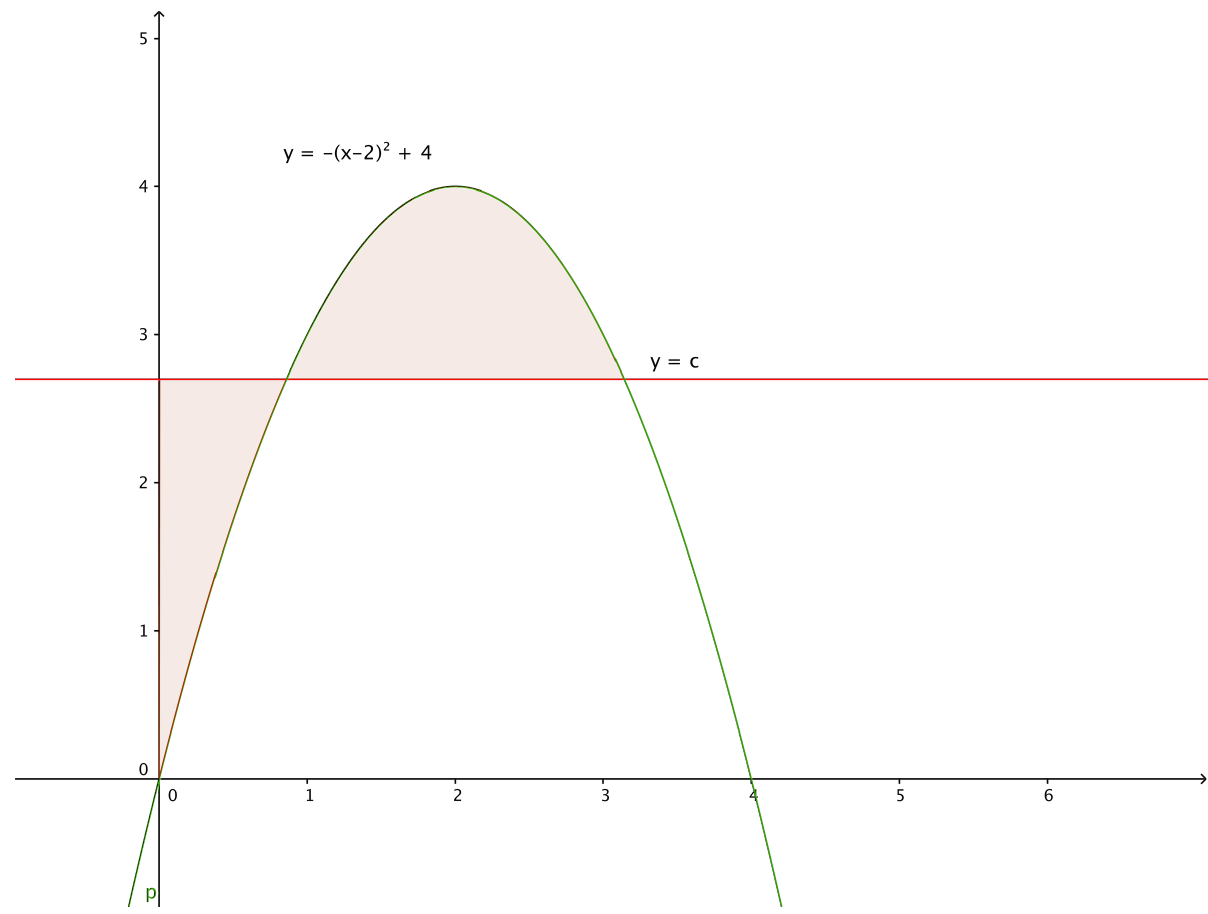
\includegraphics[width=1.2\textwidth]{seven.PNG}
\end{figure}	


\end{enumerate}

\end{document}
